\documentclass[twoside]{book}

% Packages required by doxygen
\usepackage{fixltx2e}
\usepackage{calc}
\usepackage{doxygen}
\usepackage[export]{adjustbox} % also loads graphicx
\usepackage{graphicx}
\usepackage[utf8]{inputenc}
\usepackage{makeidx}
\usepackage{multicol}
\usepackage{multirow}
\PassOptionsToPackage{warn}{textcomp}
\usepackage{textcomp}
\usepackage[nointegrals]{wasysym}
\usepackage[table]{xcolor}

% Font selection
\usepackage[T1]{fontenc}
\usepackage[scaled=.90]{helvet}
\usepackage{courier}
\usepackage{amssymb}
\usepackage{sectsty}
\renewcommand{\familydefault}{\sfdefault}
\allsectionsfont{%
  \fontseries{bc}\selectfont%
  \color{darkgray}%
}
\renewcommand{\DoxyLabelFont}{%
  \fontseries{bc}\selectfont%
  \color{darkgray}%
}
\newcommand{\+}{\discretionary{\mbox{\scriptsize$\hookleftarrow$}}{}{}}

% Page & text layout
\usepackage{geometry}
\geometry{%
  a4paper,%
  top=2.5cm,%
  bottom=2.5cm,%
  left=2.5cm,%
  right=2.5cm%
}
\tolerance=750
\hfuzz=15pt
\hbadness=750
\setlength{\emergencystretch}{15pt}
\setlength{\parindent}{0cm}
\setlength{\parskip}{0.2cm}
\makeatletter
\renewcommand{\paragraph}{%
  \@startsection{paragraph}{4}{0ex}{-1.0ex}{1.0ex}{%
    \normalfont\normalsize\bfseries\SS@parafont%
  }%
}
\renewcommand{\subparagraph}{%
  \@startsection{subparagraph}{5}{0ex}{-1.0ex}{1.0ex}{%
    \normalfont\normalsize\bfseries\SS@subparafont%
  }%
}
\makeatother

% Headers & footers
\usepackage{fancyhdr}
\pagestyle{fancyplain}
\fancyhead[LE]{\fancyplain{}{\bfseries\thepage}}
\fancyhead[CE]{\fancyplain{}{}}
\fancyhead[RE]{\fancyplain{}{\bfseries\leftmark}}
\fancyhead[LO]{\fancyplain{}{\bfseries\rightmark}}
\fancyhead[CO]{\fancyplain{}{}}
\fancyhead[RO]{\fancyplain{}{\bfseries\thepage}}
\fancyfoot[LE]{\fancyplain{}{}}
\fancyfoot[CE]{\fancyplain{}{}}
\fancyfoot[RE]{\fancyplain{}{\bfseries\scriptsize Generated on Fri Jan 9 2015 20\+:50\+:16 for Election Authority by Doxygen }}
\fancyfoot[LO]{\fancyplain{}{\bfseries\scriptsize Generated on Fri Jan 9 2015 20\+:50\+:16 for Election Authority by Doxygen }}
\fancyfoot[CO]{\fancyplain{}{}}
\fancyfoot[RO]{\fancyplain{}{}}
\renewcommand{\footrulewidth}{0.4pt}
\renewcommand{\chaptermark}[1]{%
  \markboth{#1}{}%
}
\renewcommand{\sectionmark}[1]{%
  \markright{\thesection\ #1}%
}

% Indices & bibliography
\usepackage{natbib}
\usepackage[titles]{tocloft}
\setcounter{tocdepth}{3}
\setcounter{secnumdepth}{5}
\makeindex

% Hyperlinks (required, but should be loaded last)
\usepackage{ifpdf}
\ifpdf
  \usepackage[pdftex,pagebackref=true]{hyperref}
\else
  \usepackage[ps2pdf,pagebackref=true]{hyperref}
\fi
\hypersetup{%
  colorlinks=true,%
  linkcolor=blue,%
  citecolor=blue,%
  unicode%
}

% Custom commands
\newcommand{\clearemptydoublepage}{%
  \newpage{\pagestyle{empty}\cleardoublepage}%
}


%===== C O N T E N T S =====

\begin{document}

% Titlepage & ToC
\hypersetup{pageanchor=false,
             bookmarks=true,
             bookmarksnumbered=true,
             pdfencoding=unicode
            }
\pagenumbering{roman}
\begin{titlepage}
\vspace*{7cm}
\begin{center}%
{\Large Election Authority }\\
\vspace*{1cm}
{\large Generated by Doxygen 1.8.9.1}\\
\vspace*{0.5cm}
{\small Fri Jan 9 2015 20:50:16}\\
\end{center}
\end{titlepage}
\clearemptydoublepage
\tableofcontents
\clearemptydoublepage
\pagenumbering{arabic}
\hypersetup{pageanchor=true}

%--- Begin generated contents ---
\chapter{Namespace Index}
\section{Namespace List}
Here is a list of all documented namespaces with brief descriptions\+:\begin{DoxyCompactList}
\item\contentsline{section}{\hyperlink{namespace_voter}{Voter} }{\pageref{namespace_voter}}{}
\end{DoxyCompactList}

\chapter{Hierarchical Index}
\section{Class Hierarchy}
This inheritance list is sorted roughly, but not completely, alphabetically\+:\begin{DoxyCompactList}
\item \contentsline{section}{Election\+Authority.\+Auditor}{\pageref{class_election_authority_1_1_auditor}}{}
\item \contentsline{section}{Election\+Authority.\+Ballot}{\pageref{class_election_authority_1_1_ballot}}{}
\item \contentsline{section}{Election\+Authority.\+Candidate\+List}{\pageref{class_election_authority_1_1_candidate_list}}{}
\item \contentsline{section}{Election\+Authority.\+Configuration}{\pageref{class_election_authority_1_1_configuration}}{}
\item \contentsline{section}{Election\+Authority.\+Constants}{\pageref{class_election_authority_1_1_constants}}{}
\item \contentsline{section}{Election\+Authority.\+Election\+Authority}{\pageref{class_election_authority_1_1_election_authority}}{}
\item Form\begin{DoxyCompactList}
\item \contentsline{section}{Election\+Authority.\+Form1}{\pageref{class_election_authority_1_1_form1}}{}
\end{DoxyCompactList}
\item \contentsline{section}{Election\+Authority.\+Logs}{\pageref{class_election_authority_1_1_logs}}{}
\item \contentsline{section}{Election\+Authority.\+Parser}{\pageref{class_election_authority_1_1_parser}}{}
\item \contentsline{section}{Election\+Authority.\+Permutation}{\pageref{class_election_authority_1_1_permutation}}{}
\item \contentsline{section}{Election\+Authority.\+Serial\+Number\+Generator}{\pageref{class_election_authority_1_1_serial_number_generator}}{}
\item \contentsline{section}{Election\+Authority.\+Server}{\pageref{class_election_authority_1_1_server}}{}
\end{DoxyCompactList}

\chapter{Class Index}
\section{Class List}
Here are the classes, structs, unions and interfaces with brief descriptions\+:\begin{DoxyCompactList}
\item\contentsline{section}{\hyperlink{class_voter_1_1_client}{Voter.\+Client} }{\pageref{class_voter_1_1_client}}{}
\item\contentsline{section}{\hyperlink{class_voter_1_1_configuration}{Voter.\+Configuration} \\*loading config from file }{\pageref{class_voter_1_1_configuration}}{}
\item\contentsline{section}{\hyperlink{class_voter_1_1_confirmation}{Voter.\+Confirmation} \\*confirmation for voter -\/ proxy sends him this column which he/she has choosen (precisely signed, explicit and token) }{\pageref{class_voter_1_1_confirmation}}{}
\item\contentsline{section}{\hyperlink{class_voter_1_1_constants}{Voter.\+Constants} \\*constants used in project }{\pageref{class_voter_1_1_constants}}{}
\item\contentsline{section}{\hyperlink{class_voter_1_1_form1}{Voter.\+Form1} \\*graphical user interface }{\pageref{class_voter_1_1_form1}}{}
\item\contentsline{section}{\hyperlink{class_voter_1_1_logs}{Voter.\+Logs} \\*allows to collect and display logs }{\pageref{class_voter_1_1_logs}}{}
\item\contentsline{section}{\hyperlink{class_voter_1_1_parser}{Voter.\+Parser} \\*parsing recived messages }{\pageref{class_voter_1_1_parser}}{}
\item\contentsline{section}{\hyperlink{class_voter_1_1_voter}{Voter.\+Voter} \\*\hyperlink{class_voter_1_1_voter}{Voter} class -\/ getting vote from person }{\pageref{class_voter_1_1_voter}}{}
\item\contentsline{section}{\hyperlink{class_voter_1_1_voter_ballot}{Voter.\+Voter\+Ballot} \\*\hyperlink{class_voter_1_1_voter}{Voter} ballot (vote\textquotesingle{}s data as S\+L, S\+R, vote, yes/no position) }{\pageref{class_voter_1_1_voter_ballot}}{}
\end{DoxyCompactList}

\chapter{Namespace Documentation}
\hypertarget{namespace_election_authority}{}\section{Package Election\+Authority}
\label{namespace_election_authority}\index{Election\+Authority@{Election\+Authority}}
\subsection*{Classes}
\begin{DoxyCompactItemize}
\item 
class \hyperlink{class_election_authority_1_1_auditor}{Auditor}
\begin{DoxyCompactList}\small\item\em class is used to verify if E\+A did not cheat \end{DoxyCompactList}\item 
class \hyperlink{class_election_authority_1_1_ballot}{Ballot}
\begin{DoxyCompactList}\small\item\em class represents one ballot and has information about it \end{DoxyCompactList}\item 
class \hyperlink{class_election_authority_1_1_candidate_list}{Candidate\+List}
\begin{DoxyCompactList}\small\item\em class loads candidate list from txt file \end{DoxyCompactList}\item 
class \hyperlink{class_election_authority_1_1_configuration}{Configuration}
\begin{DoxyCompactList}\small\item\em loading config from txt file \end{DoxyCompactList}\item 
class \hyperlink{class_election_authority_1_1_constants}{Constants}
\begin{DoxyCompactList}\small\item\em \hyperlink{class_election_authority_1_1_constants}{Constants} used in project \end{DoxyCompactList}\item 
class \hyperlink{class_election_authority_1_1_election_authority}{Election\+Authority}
\begin{DoxyCompactList}\small\item\em Election authority class -\/ responsible for generating serial numbers(\+S\+L, S\+R and numbers connected to them) and counting votes; main class in e-\/voting project \end{DoxyCompactList}\item 
class {\bfseries Extentions}
\begin{DoxyCompactList}\small\item\em additional function for our program \end{DoxyCompactList}\item 
class \hyperlink{class_election_authority_1_1_form1}{Form1}
\begin{DoxyCompactList}\small\item\em Class which shows a G\+U\+I \end{DoxyCompactList}\item 
class \hyperlink{class_election_authority_1_1_logs}{Logs}
\begin{DoxyCompactList}\small\item\em allows to collect and display logs \end{DoxyCompactList}\item 
class \hyperlink{class_election_authority_1_1_parser}{Parser}
\begin{DoxyCompactList}\small\item\em parsing messages recived form clients \end{DoxyCompactList}\item 
class \hyperlink{class_election_authority_1_1_permutation}{Permutation}
\begin{DoxyCompactList}\small\item\em represents all permutation\textquotesingle{}s method \end{DoxyCompactList}\item 
class {\bfseries Program}
\item 
class \hyperlink{class_election_authority_1_1_serial_number_generator}{Serial\+Number\+Generator}
\begin{DoxyCompactList}\small\item\em Generates serial numbers used in E\+A \end{DoxyCompactList}\item 
class \hyperlink{class_election_authority_1_1_server}{Server}
\end{DoxyCompactItemize}

\chapter{Class Documentation}
\hypertarget{class_election_authority_1_1_auditor}{}\section{Election\+Authority.\+Auditor Class Reference}
\label{class_election_authority_1_1_auditor}\index{Election\+Authority.\+Auditor@{Election\+Authority.\+Auditor}}


class is used to verify if E\+A did not cheat  


\subsection*{Public Member Functions}
\begin{DoxyCompactItemize}
\item 
\hyperlink{class_election_authority_1_1_auditor_ad1edb55058d499d307618a0c5842b12d}{Auditor} (\hyperlink{class_election_authority_1_1_logs}{Logs} logs)
\begin{DoxyCompactList}\small\item\em \hyperlink{class_election_authority_1_1_auditor}{Auditor}\textquotesingle{}s constructor \end{DoxyCompactList}\item 
bool \hyperlink{class_election_authority_1_1_auditor_a6c3c9a569074bd3dcf5d946046a618e4}{check\+Permutation} (Rsa\+Key\+Parameters private\+Key, Rsa\+Key\+Parameters public\+Key, Big\+Integer\mbox{[}$\,$\mbox{]} explicit\+Permutation)
\begin{DoxyCompactList}\small\item\em checking the correctness of permutation \end{DoxyCompactList}\end{DoxyCompactItemize}
\subsection*{Properties}
\begin{DoxyCompactItemize}
\item 
Big\+Integer\mbox{[}$\,$\mbox{]} \hyperlink{class_election_authority_1_1_auditor_a5448d8d3151a043fd123ceba17c2329b}{Commited\+Permatation}\hspace{0.3cm}{\ttfamily  \mbox{[}get, set\mbox{]}}
\begin{DoxyCompactList}\small\item\em set and get commited permutation \end{DoxyCompactList}\end{DoxyCompactItemize}


\subsection{Detailed Description}
class is used to verify if E\+A did not cheat 



\subsection{Constructor \& Destructor Documentation}
\hypertarget{class_election_authority_1_1_auditor_ad1edb55058d499d307618a0c5842b12d}{}\index{Election\+Authority\+::\+Auditor@{Election\+Authority\+::\+Auditor}!Auditor@{Auditor}}
\index{Auditor@{Auditor}!Election\+Authority\+::\+Auditor@{Election\+Authority\+::\+Auditor}}
\subsubsection[{Auditor}]{\setlength{\rightskip}{0pt plus 5cm}Election\+Authority.\+Auditor.\+Auditor (
\begin{DoxyParamCaption}
\item[{{\bf Logs}}]{logs}
\end{DoxyParamCaption}
)\hspace{0.3cm}{\ttfamily [inline]}}\label{class_election_authority_1_1_auditor_ad1edb55058d499d307618a0c5842b12d}


\hyperlink{class_election_authority_1_1_auditor}{Auditor}\textquotesingle{}s constructor 


\begin{DoxyParams}{Parameters}
{\em logs} & transfered log instance \\
\hline
\end{DoxyParams}


\subsection{Member Function Documentation}
\hypertarget{class_election_authority_1_1_auditor_a6c3c9a569074bd3dcf5d946046a618e4}{}\index{Election\+Authority\+::\+Auditor@{Election\+Authority\+::\+Auditor}!check\+Permutation@{check\+Permutation}}
\index{check\+Permutation@{check\+Permutation}!Election\+Authority\+::\+Auditor@{Election\+Authority\+::\+Auditor}}
\subsubsection[{check\+Permutation}]{\setlength{\rightskip}{0pt plus 5cm}bool Election\+Authority.\+Auditor.\+check\+Permutation (
\begin{DoxyParamCaption}
\item[{Rsa\+Key\+Parameters}]{private\+Key, }
\item[{Rsa\+Key\+Parameters}]{public\+Key, }
\item[{Big\+Integer\mbox{[}$\,$\mbox{]}}]{explicit\+Permutation}
\end{DoxyParamCaption}
)\hspace{0.3cm}{\ttfamily [inline]}}\label{class_election_authority_1_1_auditor_a6c3c9a569074bd3dcf5d946046a618e4}


checking the correctness of permutation 


\begin{DoxyParams}{Parameters}
{\em private\+Key} & private key used for bit commitment\\
\hline
{\em public\+Key} & public key used for bit commitment\\
\hline
{\em explicit\+Permutation} & used permutation (as open text)\\
\hline
\end{DoxyParams}
\begin{DoxyReturn}{Returns}

\end{DoxyReturn}


\subsection{Property Documentation}
\hypertarget{class_election_authority_1_1_auditor_a5448d8d3151a043fd123ceba17c2329b}{}\index{Election\+Authority\+::\+Auditor@{Election\+Authority\+::\+Auditor}!Commited\+Permatation@{Commited\+Permatation}}
\index{Commited\+Permatation@{Commited\+Permatation}!Election\+Authority\+::\+Auditor@{Election\+Authority\+::\+Auditor}}
\subsubsection[{Commited\+Permatation}]{\setlength{\rightskip}{0pt plus 5cm}Big\+Integer \mbox{[}$\,$\mbox{]} Election\+Authority.\+Auditor.\+Commited\+Permatation\hspace{0.3cm}{\ttfamily [get]}, {\ttfamily [set]}}\label{class_election_authority_1_1_auditor_a5448d8d3151a043fd123ceba17c2329b}


set and get commited permutation 



The documentation for this class was generated from the following file\+:\begin{DoxyCompactItemize}
\item 
Election\+Authority/\+Election\+Authority/Auditor.\+cs\end{DoxyCompactItemize}

\hypertarget{class_election_authority_1_1_ballot}{}\section{Election\+Authority.\+Ballot Class Reference}
\label{class_election_authority_1_1_ballot}\index{Election\+Authority.\+Ballot@{Election\+Authority.\+Ballot}}


class represents one ballot and has information about it  


\subsection*{Public Member Functions}
\begin{DoxyCompactItemize}
\item 
\hyperlink{class_election_authority_1_1_ballot_adf2bd5aa976f9621fbf41be8dc90cde3}{Ballot} (Big\+Integer S\+L)
\begin{DoxyCompactList}\small\item\em ballot\textquotesingle{}s constructor \end{DoxyCompactList}\item 
void \hyperlink{class_election_authority_1_1_ballot_a46f6344c3df065147f3e5ea96ced555e}{sign\+Column} ()
\begin{DoxyCompactList}\small\item\em Method to sing each column in ballot\+Matrix \end{DoxyCompactList}\end{DoxyCompactItemize}
\subsection*{Properties}
\begin{DoxyCompactItemize}
\item 
\hypertarget{class_election_authority_1_1_ballot_a528eb06838f7ac22b1247382aba42a44}{}Big\+Integer {\bfseries S\+L}\hspace{0.3cm}{\ttfamily  \mbox{[}get\mbox{]}}\label{class_election_authority_1_1_ballot_a528eb06838f7ac22b1247382aba42a44}

\item 
\hypertarget{class_election_authority_1_1_ballot_af287c51b6ef66dc68660223e049e6fd2}{}List$<$ Big\+Integer $>$ {\bfseries Token\+List}\hspace{0.3cm}{\ttfamily  \mbox{[}get, set\mbox{]}}\label{class_election_authority_1_1_ballot_af287c51b6ef66dc68660223e049e6fd2}

\item 
\hypertarget{class_election_authority_1_1_ballot_acbc5a267fbb7061b30b75fdf4b6ff732}{}List$<$ Big\+Integer $>$ {\bfseries Exponents\+List}\hspace{0.3cm}{\ttfamily  \mbox{[}get, set\mbox{]}}\label{class_election_authority_1_1_ballot_acbc5a267fbb7061b30b75fdf4b6ff732}

\item 
\hypertarget{class_election_authority_1_1_ballot_a6e0ac0cec03b599222078e27c00ea407}{}List$<$ Big\+Integer $>$ {\bfseries Signature\+Factor}\hspace{0.3cm}{\ttfamily  \mbox{[}get, set\mbox{]}}\label{class_election_authority_1_1_ballot_a6e0ac0cec03b599222078e27c00ea407}

\item 
\hypertarget{class_election_authority_1_1_ballot_a12f22d693875711956628ce658a7c7a1}{}Big\+Integer\mbox{[}$\,$\mbox{]} {\bfseries Signed\+Column}\hspace{0.3cm}{\ttfamily  \mbox{[}get\mbox{]}}\label{class_election_authority_1_1_ballot_a12f22d693875711956628ce658a7c7a1}

\item 
\hypertarget{class_election_authority_1_1_ballot_a478ff6455f8988f2ca215e4e42ac99b1}{}Big\+Integer\mbox{[}$\,$\mbox{]} {\bfseries Blind\+Column}\hspace{0.3cm}{\ttfamily  \mbox{[}set\mbox{]}}\label{class_election_authority_1_1_ballot_a478ff6455f8988f2ca215e4e42ac99b1}

\item 
\hypertarget{class_election_authority_1_1_ballot_a845f82b655115b96b8fea01b71a286a5}{}string\mbox{[},\mbox{]} {\bfseries Unblinded\+Ballot}\hspace{0.3cm}{\ttfamily  \mbox{[}get, set\mbox{]}}\label{class_election_authority_1_1_ballot_a845f82b655115b96b8fea01b71a286a5}

\item 
\hypertarget{class_election_authority_1_1_ballot_a2c269eed9da76c0d94e776cf092b5590}{}List$<$ Big\+Integer $>$ {\bfseries Permutation}\hspace{0.3cm}{\ttfamily  \mbox{[}get, set\mbox{]}}\label{class_election_authority_1_1_ballot_a2c269eed9da76c0d94e776cf092b5590}

\item 
\hypertarget{class_election_authority_1_1_ballot_a0b3aa5510c43a3b0cc5601eafd75b946}{}List$<$ Big\+Integer $>$ {\bfseries Inverse\+Permutation}\hspace{0.3cm}{\ttfamily  \mbox{[}get, set\mbox{]}}\label{class_election_authority_1_1_ballot_a0b3aa5510c43a3b0cc5601eafd75b946}

\end{DoxyCompactItemize}


\subsection{Detailed Description}
class represents one ballot and has information about it 



\subsection{Constructor \& Destructor Documentation}
\hypertarget{class_election_authority_1_1_ballot_adf2bd5aa976f9621fbf41be8dc90cde3}{}\index{Election\+Authority\+::\+Ballot@{Election\+Authority\+::\+Ballot}!Ballot@{Ballot}}
\index{Ballot@{Ballot}!Election\+Authority\+::\+Ballot@{Election\+Authority\+::\+Ballot}}
\subsubsection[{Ballot}]{\setlength{\rightskip}{0pt plus 5cm}Election\+Authority.\+Ballot.\+Ballot (
\begin{DoxyParamCaption}
\item[{Big\+Integer}]{S\+L}
\end{DoxyParamCaption}
)\hspace{0.3cm}{\ttfamily [inline]}}\label{class_election_authority_1_1_ballot_adf2bd5aa976f9621fbf41be8dc90cde3}


ballot\textquotesingle{}s constructor 


\begin{DoxyParams}{Parameters}
{\em S\+L} & serial (list of candidate) number\\
\hline
\end{DoxyParams}


\subsection{Member Function Documentation}
\hypertarget{class_election_authority_1_1_ballot_a46f6344c3df065147f3e5ea96ced555e}{}\index{Election\+Authority\+::\+Ballot@{Election\+Authority\+::\+Ballot}!sign\+Column@{sign\+Column}}
\index{sign\+Column@{sign\+Column}!Election\+Authority\+::\+Ballot@{Election\+Authority\+::\+Ballot}}
\subsubsection[{sign\+Column}]{\setlength{\rightskip}{0pt plus 5cm}void Election\+Authority.\+Ballot.\+sign\+Column (
\begin{DoxyParamCaption}
{}
\end{DoxyParamCaption}
)\hspace{0.3cm}{\ttfamily [inline]}}\label{class_election_authority_1_1_ballot_a46f6344c3df065147f3e5ea96ced555e}


Method to sing each column in ballot\+Matrix 



The documentation for this class was generated from the following file\+:\begin{DoxyCompactItemize}
\item 
Election\+Authority/\+Election\+Authority/Ballot.\+cs\end{DoxyCompactItemize}

\hypertarget{class_election_authority_1_1_candidate_list}{}\section{Election\+Authority.\+Candidate\+List Class Reference}
\label{class_election_authority_1_1_candidate_list}\index{Election\+Authority.\+Candidate\+List@{Election\+Authority.\+Candidate\+List}}


class loads candidate list from txt file  


\subsection*{Public Member Functions}
\begin{DoxyCompactItemize}
\item 
\hyperlink{class_election_authority_1_1_candidate_list_abd9114612080354d3b549e988421d53f}{Candidate\+List} (\hyperlink{class_election_authority_1_1_logs}{Logs} logs)
\begin{DoxyCompactList}\small\item\em condidate list constructor \end{DoxyCompactList}\item 
List$<$ string $>$ \hyperlink{class_election_authority_1_1_candidate_list_ad4bbc38420fb19a72842a8f3741a3800}{load\+Canidate\+List} (string path)
\begin{DoxyCompactList}\small\item\em loading cadidate list \end{DoxyCompactList}\item 
string \hyperlink{class_election_authority_1_1_candidate_list_a37406221224e2b20f6f76ca774b70a47}{get\+Path\+To\+Candidate\+List} (string path)
\begin{DoxyCompactList}\small\item\em gets path to txt file with candidates list \end{DoxyCompactList}\end{DoxyCompactItemize}


\subsection{Detailed Description}
class loads candidate list from txt file 



\subsection{Constructor \& Destructor Documentation}
\hypertarget{class_election_authority_1_1_candidate_list_abd9114612080354d3b549e988421d53f}{}\index{Election\+Authority\+::\+Candidate\+List@{Election\+Authority\+::\+Candidate\+List}!Candidate\+List@{Candidate\+List}}
\index{Candidate\+List@{Candidate\+List}!Election\+Authority\+::\+Candidate\+List@{Election\+Authority\+::\+Candidate\+List}}
\subsubsection[{Candidate\+List}]{\setlength{\rightskip}{0pt plus 5cm}Election\+Authority.\+Candidate\+List.\+Candidate\+List (
\begin{DoxyParamCaption}
\item[{{\bf Logs}}]{logs}
\end{DoxyParamCaption}
)\hspace{0.3cm}{\ttfamily [inline]}}\label{class_election_authority_1_1_candidate_list_abd9114612080354d3b549e988421d53f}


condidate list constructor 


\begin{DoxyParams}{Parameters}
{\em logs} & logs instance\\
\hline
\end{DoxyParams}


\subsection{Member Function Documentation}
\hypertarget{class_election_authority_1_1_candidate_list_a37406221224e2b20f6f76ca774b70a47}{}\index{Election\+Authority\+::\+Candidate\+List@{Election\+Authority\+::\+Candidate\+List}!get\+Path\+To\+Candidate\+List@{get\+Path\+To\+Candidate\+List}}
\index{get\+Path\+To\+Candidate\+List@{get\+Path\+To\+Candidate\+List}!Election\+Authority\+::\+Candidate\+List@{Election\+Authority\+::\+Candidate\+List}}
\subsubsection[{get\+Path\+To\+Candidate\+List}]{\setlength{\rightskip}{0pt plus 5cm}string Election\+Authority.\+Candidate\+List.\+get\+Path\+To\+Candidate\+List (
\begin{DoxyParamCaption}
\item[{string}]{path}
\end{DoxyParamCaption}
)\hspace{0.3cm}{\ttfamily [inline]}}\label{class_election_authority_1_1_candidate_list_a37406221224e2b20f6f76ca774b70a47}


gets path to txt file with candidates list 


\begin{DoxyParams}{Parameters}
{\em path} & path to txt file\\
\hline
\end{DoxyParams}
\begin{DoxyReturn}{Returns}
path to file
\end{DoxyReturn}
\hypertarget{class_election_authority_1_1_candidate_list_ad4bbc38420fb19a72842a8f3741a3800}{}\index{Election\+Authority\+::\+Candidate\+List@{Election\+Authority\+::\+Candidate\+List}!load\+Canidate\+List@{load\+Canidate\+List}}
\index{load\+Canidate\+List@{load\+Canidate\+List}!Election\+Authority\+::\+Candidate\+List@{Election\+Authority\+::\+Candidate\+List}}
\subsubsection[{load\+Canidate\+List}]{\setlength{\rightskip}{0pt plus 5cm}List$<$string$>$ Election\+Authority.\+Candidate\+List.\+load\+Canidate\+List (
\begin{DoxyParamCaption}
\item[{string}]{path}
\end{DoxyParamCaption}
)\hspace{0.3cm}{\ttfamily [inline]}}\label{class_election_authority_1_1_candidate_list_ad4bbc38420fb19a72842a8f3741a3800}


loading cadidate list 


\begin{DoxyParams}{Parameters}
{\em path} & path to txt file\\
\hline
\end{DoxyParams}
\begin{DoxyReturn}{Returns}
List of strings with candidates
\end{DoxyReturn}


The documentation for this class was generated from the following file\+:\begin{DoxyCompactItemize}
\item 
Election\+Authority/\+Election\+Authority/Candidate\+List.\+cs\end{DoxyCompactItemize}

\hypertarget{class_election_authority_1_1_configuration}{}\section{Election\+Authority.\+Configuration Class Reference}
\label{class_election_authority_1_1_configuration}\index{Election\+Authority.\+Configuration@{Election\+Authority.\+Configuration}}


loading config from txt file  


\subsection*{Public Member Functions}
\begin{DoxyCompactItemize}
\item 
\hypertarget{class_election_authority_1_1_configuration_a6fbd2e89ab14280ab3a676cca7477cfd}{}{\bfseries Configuration} (\hyperlink{class_election_authority_1_1_logs}{Logs} logs)\label{class_election_authority_1_1_configuration_a6fbd2e89ab14280ab3a676cca7477cfd}

\item 
\hypertarget{class_election_authority_1_1_configuration_a97aa848259fc5132ec80672c90951815}{}bool {\bfseries load\+Configuration} (string path)\label{class_election_authority_1_1_configuration_a97aa848259fc5132ec80672c90951815}

\end{DoxyCompactItemize}
\subsection*{Properties}
\begin{DoxyCompactItemize}
\item 
\hypertarget{class_election_authority_1_1_configuration_ac7c904d1ab2e25b350016093f0f51e17}{}string {\bfseries Election\+Authority\+I\+D}\hspace{0.3cm}{\ttfamily  \mbox{[}get\mbox{]}}\label{class_election_authority_1_1_configuration_ac7c904d1ab2e25b350016093f0f51e17}

\item 
\hypertarget{class_election_authority_1_1_configuration_a4d2632fc7e7a8351f5f392c1e7e20cc1}{}string {\bfseries Election\+Authority\+Port\+Client}\hspace{0.3cm}{\ttfamily  \mbox{[}get\mbox{]}}\label{class_election_authority_1_1_configuration_a4d2632fc7e7a8351f5f392c1e7e20cc1}

\item 
\hypertarget{class_election_authority_1_1_configuration_a560f3427f69d9c845b07ee06684c3530}{}string {\bfseries Election\+Authority\+Port\+Proxy}\hspace{0.3cm}{\ttfamily  \mbox{[}get\mbox{]}}\label{class_election_authority_1_1_configuration_a560f3427f69d9c845b07ee06684c3530}

\item 
\hypertarget{class_election_authority_1_1_configuration_ae581a3a4b33a68b9fdfd62858ce6d1ab}{}string {\bfseries Number\+Of\+Voters}\hspace{0.3cm}{\ttfamily  \mbox{[}get\mbox{]}}\label{class_election_authority_1_1_configuration_ae581a3a4b33a68b9fdfd62858ce6d1ab}

\end{DoxyCompactItemize}


\subsection{Detailed Description}
loading config from txt file 



The documentation for this class was generated from the following file\+:\begin{DoxyCompactItemize}
\item 
Election\+Authority/\+Election\+Authority/Configuration.\+cs\end{DoxyCompactItemize}

\hypertarget{class_election_authority_1_1_constants}{}\section{Election\+Authority.\+Constants Class Reference}
\label{class_election_authority_1_1_constants}\index{Election\+Authority.\+Constants@{Election\+Authority.\+Constants}}


\hyperlink{class_election_authority_1_1_constants}{Constants} used in project  


\subsection*{Public Attributes}
\begin{DoxyCompactItemize}
\item 
\hypertarget{class_election_authority_1_1_constants_a8307e0c5c711b7fb8e914d9ae29ddbb7}{}const int {\bfseries B\+A\+L\+L\+O\+T\+\_\+\+S\+I\+Z\+E} = 4\label{class_election_authority_1_1_constants_a8307e0c5c711b7fb8e914d9ae29ddbb7}

\item 
\hypertarget{class_election_authority_1_1_constants_a0f3935d2e5afe19da922aa9764417779}{}const int {\bfseries L\+O\+G\+\_\+\+I\+N\+F\+O} = 0\label{class_election_authority_1_1_constants_a0f3935d2e5afe19da922aa9764417779}

\item 
\hypertarget{class_election_authority_1_1_constants_a1b3b302c031ce27192fdfc4d1bcce966}{}const int {\bfseries L\+O\+G\+\_\+\+M\+E\+S\+S\+A\+G\+E} = 1\label{class_election_authority_1_1_constants_a1b3b302c031ce27192fdfc4d1bcce966}

\item 
\hypertarget{class_election_authority_1_1_constants_a7d9e61b980d9bcd50e952c432e47f9ac}{}const int {\bfseries L\+O\+G\+\_\+\+E\+R\+R\+O\+R} = 2\label{class_election_authority_1_1_constants_a7d9e61b980d9bcd50e952c432e47f9ac}

\item 
\hypertarget{class_election_authority_1_1_constants_a666a945fb4d7c65f5af4c757efc7769d}{}const string {\bfseries I\+D} = \char`\"{}I\+D\char`\"{}\label{class_election_authority_1_1_constants_a666a945fb4d7c65f5af4c757efc7769d}

\item 
\hypertarget{class_election_authority_1_1_constants_aae8fe339cbf18c3f751be660bd958e06}{}const string {\bfseries E\+L\+E\+C\+T\+I\+O\+N\+\_\+\+A\+U\+T\+H\+O\+R\+I\+T\+Y\+\_\+\+P\+O\+R\+T\+\_\+\+C\+L\+I\+E\+N\+T} = \char`\"{}election\+Authority\+Port\+For\+Client\char`\"{}\label{class_election_authority_1_1_constants_aae8fe339cbf18c3f751be660bd958e06}

\item 
\hypertarget{class_election_authority_1_1_constants_a49313fc45be743d16fb7f75fb86a5e18}{}const string {\bfseries E\+L\+E\+C\+T\+I\+O\+N\+\_\+\+A\+U\+T\+H\+O\+R\+I\+T\+Y\+\_\+\+P\+O\+R\+T\+\_\+\+P\+R\+O\+X\+Y} = \char`\"{}election\+Authority\+Port\+For\+Proxy\char`\"{}\label{class_election_authority_1_1_constants_a49313fc45be743d16fb7f75fb86a5e18}

\item 
\hypertarget{class_election_authority_1_1_constants_a6a91d63b321505807b5fec84994022bb}{}const string {\bfseries C\+O\+N\+F\+I\+G\+U\+R\+A\+T\+I\+O\+N\+\_\+\+L\+O\+A\+D\+E\+D\+\_\+\+F\+R\+O\+M} = \char`\"{}Configuration loaded from file\+: \char`\"{}\label{class_election_authority_1_1_constants_a6a91d63b321505807b5fec84994022bb}

\item 
\hypertarget{class_election_authority_1_1_constants_a7d6511b05d035ac174ae3b0c4873bb87}{}const string {\bfseries N\+U\+M\+B\+E\+R\+\_\+\+O\+F\+\_\+\+V\+O\+T\+E\+R\+S} = \char`\"{}number\+Of\+Voters\char`\"{}\label{class_election_authority_1_1_constants_a7d6511b05d035ac174ae3b0c4873bb87}

\item 
\hypertarget{class_election_authority_1_1_constants_a3f85ebb7470065a57a7ccdf0e5ce3d35}{}const string {\bfseries P\+A\+T\+H\+\_\+\+T\+O\+\_\+\+C\+O\+N\+F\+I\+G} = @\char`\"{}Config\textbackslash{}\+Election\+Authority.\+xml\char`\"{}\label{class_election_authority_1_1_constants_a3f85ebb7470065a57a7ccdf0e5ce3d35}

\item 
\hypertarget{class_election_authority_1_1_constants_adf963e0f80abbb8087eb47063a1a5317}{}const string {\bfseries C\+A\+N\+D\+I\+D\+A\+T\+E\+\_\+\+L\+I\+S\+T} = \char`\"{}Candidate\+List.\+xml\char`\"{}\label{class_election_authority_1_1_constants_adf963e0f80abbb8087eb47063a1a5317}

\item 
\hypertarget{class_election_authority_1_1_constants_aea5ac2a751a33e363c9e6b4438458319}{}const string {\bfseries S\+E\+R\+V\+E\+R\+\_\+\+S\+T\+A\+R\+T\+E\+D\+\_\+\+C\+O\+R\+R\+E\+C\+T\+L\+Y} = \char`\"{}Election Authority started working correctly\char`\"{}\label{class_election_authority_1_1_constants_aea5ac2a751a33e363c9e6b4438458319}

\item 
\hypertarget{class_election_authority_1_1_constants_af9e8ce72d3248d5c45e05c4b94f37bf2}{}const string {\bfseries S\+E\+R\+V\+E\+R\+\_\+\+U\+N\+A\+B\+L\+E\+\_\+\+T\+O\+\_\+\+S\+T\+A\+R\+T} = \char`\"{}Election Authority unable to start working\char`\"{}\label{class_election_authority_1_1_constants_af9e8ce72d3248d5c45e05c4b94f37bf2}

\item 
\hypertarget{class_election_authority_1_1_constants_adabf1df04f349b967455b9516e5d5d05}{}const string {\bfseries U\+N\+K\+N\+O\+W\+N} = \char`\"{}Unknown\char`\"{}\label{class_election_authority_1_1_constants_adabf1df04f349b967455b9516e5d5d05}

\item 
\hypertarget{class_election_authority_1_1_constants_af1f1f5dfffb44c80db736ebd95e06f45}{}const string {\bfseries D\+I\+S\+C\+O\+N\+N\+E\+C\+T\+E\+D\+\_\+\+N\+O\+D\+E} = \char`\"{}Someone has been disconnected\char`\"{}\label{class_election_authority_1_1_constants_af1f1f5dfffb44c80db736ebd95e06f45}

\item 
\hypertarget{class_election_authority_1_1_constants_a3443667b831e187da3aa6753b5573b09}{}const string {\bfseries C\+A\+N\+D\+I\+D\+A\+T\+E\+\_\+\+L\+I\+S\+T\+\_\+\+S\+U\+C\+C\+E\+S\+S\+F\+U\+L} = \char`\"{}Candidate list loaded successfully\char`\"{}\label{class_election_authority_1_1_constants_a3443667b831e187da3aa6753b5573b09}

\item 
\hypertarget{class_election_authority_1_1_constants_ad320f14b6a61bfa0453fed63edc838f9}{}const string {\bfseries P\+E\+R\+M\+U\+T\+A\+T\+I\+O\+N\+\_\+\+G\+E\+N\+\_\+\+S\+U\+C\+C\+E\+S\+S\+F\+U\+L\+L\+Y} = \char`\"{}Permuration generated successfully\char`\"{}\label{class_election_authority_1_1_constants_ad320f14b6a61bfa0453fed63edc838f9}

\item 
\hypertarget{class_election_authority_1_1_constants_a21e0559abddd3774ff20f69de0c5a549}{}const string {\bfseries S\+E\+R\+I\+A\+L\+\_\+\+N\+U\+M\+B\+E\+R\+\_\+\+G\+E\+N\+\_\+\+S\+U\+C\+C\+E\+S\+S\+F\+U\+L\+L\+Y} = \char`\"{}Serial number list generated successfully\char`\"{}\label{class_election_authority_1_1_constants_a21e0559abddd3774ff20f69de0c5a549}

\item 
\hypertarget{class_election_authority_1_1_constants_abb781de9ffb55e466656b49a850a4b43}{}const string {\bfseries S\+L\+\_\+\+C\+O\+N\+N\+E\+C\+T\+E\+D\+\_\+\+W\+I\+T\+H\+\_\+\+P\+E\+R\+M\+U\+T\+A\+T\+I\+O\+N} = \char`\"{}Serial numbers connected with permutation\char`\"{}\label{class_election_authority_1_1_constants_abb781de9ffb55e466656b49a850a4b43}

\item 
\hypertarget{class_election_authority_1_1_constants_a00f65992a14512d2399946eb9af7e2b0}{}const int {\bfseries N\+U\+M\+B\+E\+R\+\_\+\+O\+F\+\_\+\+B\+I\+T\+S\+\_\+\+S\+L} = 64\label{class_election_authority_1_1_constants_a00f65992a14512d2399946eb9af7e2b0}

\item 
\hypertarget{class_election_authority_1_1_constants_a46feadcc571278025f21b29ed0f9c89c}{}const int {\bfseries N\+U\+M\+B\+E\+R\+\_\+\+O\+F\+\_\+\+T\+O\+K\+E\+N\+S} = 4\label{class_election_authority_1_1_constants_a46feadcc571278025f21b29ed0f9c89c}

\item 
\hypertarget{class_election_authority_1_1_constants_a2f27187ba8d2e211dcc1e71bafb1f153}{}const string {\bfseries T\+O\+K\+E\+N\+S\+\_\+\+G\+E\+N\+E\+R\+A\+T\+E\+D\+\_\+\+S\+U\+C\+C\+E\+S\+S\+F\+U\+L\+L\+Y} = \char`\"{}Tokens generated successfully\char`\"{}\label{class_election_authority_1_1_constants_a2f27187ba8d2e211dcc1e71bafb1f153}

\item 
\hypertarget{class_election_authority_1_1_constants_a42bb446aa5d8917b47a2c98893ed2ae1}{}const int {\bfseries N\+U\+M\+B\+E\+R\+\_\+\+O\+F\+\_\+\+B\+I\+T\+S\+\_\+\+T\+O\+K\+E\+N} =512\label{class_election_authority_1_1_constants_a42bb446aa5d8917b47a2c98893ed2ae1}

\item 
\hypertarget{class_election_authority_1_1_constants_af30758e38d2e4ff6d10f071b039d92a6}{}const string {\bfseries S\+L\+\_\+\+C\+O\+N\+N\+E\+C\+T\+E\+D\+\_\+\+W\+I\+T\+H\+\_\+\+T\+O\+K\+E\+N\+S} = \char`\"{}Serial numbers connected with tokens\char`\"{}\label{class_election_authority_1_1_constants_af30758e38d2e4ff6d10f071b039d92a6}

\item 
\hypertarget{class_election_authority_1_1_constants_adb879bc3dce48c69eec79ce0a6f499e5}{}const string {\bfseries S\+L\+\_\+\+R\+E\+C\+E\+I\+V\+E\+D\+\_\+\+S\+U\+C\+C\+E\+S\+S\+F\+U\+L\+L\+Y} = \char`\"{}S\+L\+\_\+\+R\+E\+C\+E\+I\+V\+E\+D\+\_\+\+S\+U\+C\+C\+E\+S\+S\+F\+U\+L\+L\+Y\char`\"{}\label{class_election_authority_1_1_constants_adb879bc3dce48c69eec79ce0a6f499e5}

\item 
\hypertarget{class_election_authority_1_1_constants_a2fd1053467beee8dae6266ed5c386533}{}const string {\bfseries S\+L\+\_\+\+A\+N\+D\+\_\+\+S\+R\+\_\+\+S\+E\+N\+T\+\_\+\+S\+U\+C\+C\+E\+S\+S\+F\+U\+L\+L\+Y} = \char`\"{}S\+L sent successfully to Proxy\char`\"{}\label{class_election_authority_1_1_constants_a2fd1053467beee8dae6266ed5c386533}

\item 
\hypertarget{class_election_authority_1_1_constants_a8dcfc266f9563c6f57b1c7869c4fa552}{}const string {\bfseries P\+R\+O\+X\+Y} =\char`\"{}P\+R\+O\+X\+Y\char`\"{}\label{class_election_authority_1_1_constants_a8dcfc266f9563c6f57b1c7869c4fa552}

\item 
\hypertarget{class_election_authority_1_1_constants_a6bcab0cd9bf03d0e20e585f3080e9557}{}const string {\bfseries G\+E\+T\+\_\+\+C\+A\+N\+D\+I\+D\+A\+T\+E\+\_\+\+L\+I\+S\+T} = \char`\"{}G\+E\+T\+\_\+\+C\+A\+N\+D\+I\+D\+A\+T\+E\+\_\+\+L\+I\+S\+T\char`\"{}\label{class_election_authority_1_1_constants_a6bcab0cd9bf03d0e20e585f3080e9557}

\item 
\hypertarget{class_election_authority_1_1_constants_a53cf9a84bfae1ba52085d2a8c556e683}{}const string {\bfseries C\+A\+N\+D\+I\+D\+A\+T\+E\+\_\+\+L\+I\+S\+T\+\_\+\+R\+E\+S\+P\+O\+N\+S\+E} = \char`\"{}C\+A\+N\+D\+I\+D\+A\+T\+E\+\_\+\+L\+I\+S\+T\+\_\+\+R\+E\+S\+P\+O\+N\+S\+E\char`\"{}\label{class_election_authority_1_1_constants_a53cf9a84bfae1ba52085d2a8c556e683}

\item 
\hypertarget{class_election_authority_1_1_constants_ac05b304ec6ab025cb539fd21609cd5a8}{}const string {\bfseries B\+L\+I\+N\+D\+\_\+\+P\+R\+O\+X\+Y\+\_\+\+B\+A\+L\+L\+O\+T} = \char`\"{}B\+L\+I\+N\+D\+\_\+\+P\+R\+O\+X\+Y\+\_\+\+B\+A\+L\+L\+O\+T\char`\"{}\label{class_election_authority_1_1_constants_ac05b304ec6ab025cb539fd21609cd5a8}

\item 
\hypertarget{class_election_authority_1_1_constants_af63b0c36b4ecc49583ab084d861a4e8d}{}const string {\bfseries B\+L\+I\+N\+D\+\_\+\+P\+R\+O\+X\+Y\+\_\+\+B\+A\+L\+L\+O\+T\+\_\+\+R\+E\+C\+E\+I\+V\+E\+D} = \char`\"{}Blind ballot received from voter with I\+D\+: \char`\"{}\label{class_election_authority_1_1_constants_af63b0c36b4ecc49583ab084d861a4e8d}

\item 
\hypertarget{class_election_authority_1_1_constants_af112ec6083e9fa13bd2266f0e66ecd4d}{}const string {\bfseries S\+I\+G\+N\+E\+D\+\_\+\+P\+R\+O\+X\+Y\+\_\+\+B\+A\+L\+L\+O\+T} = \char`\"{}S\+I\+G\+N\+E\+D\+\_\+\+P\+R\+O\+X\+Y\+\_\+\+B\+A\+L\+L\+O\+T\char`\"{}\label{class_election_authority_1_1_constants_af112ec6083e9fa13bd2266f0e66ecd4d}

\item 
\hypertarget{class_election_authority_1_1_constants_ae6bb23eaf3057e69dbc0451bbec0072b}{}const string {\bfseries S\+I\+G\+N\+E\+D\+\_\+\+B\+A\+L\+L\+O\+T\+\_\+\+M\+A\+T\+R\+I\+X\+\_\+\+S\+E\+N\+T} = \char`\"{}S\+I\+G\+N\+E\+D\+\_\+\+B\+A\+L\+L\+O\+T\+\_\+\+M\+A\+T\+R\+I\+X\+\_\+\+S\+E\+N\+T\char`\"{}\label{class_election_authority_1_1_constants_ae6bb23eaf3057e69dbc0451bbec0072b}

\item 
\hypertarget{class_election_authority_1_1_constants_ad3c8d542cac9f7bf74257b153f1c31b2}{}const string {\bfseries G\+E\+N\+E\+R\+A\+T\+E\+\_\+\+I\+N\+V\+E\+R\+S\+E\+\_\+\+P\+E\+R\+M\+U\+T\+A\+T\+I\+O\+N} = \char`\"{}Inverse permutation generated\char`\"{}\label{class_election_authority_1_1_constants_ad3c8d542cac9f7bf74257b153f1c31b2}

\item 
\hypertarget{class_election_authority_1_1_constants_a9ee35e14bf4be6841cc7a2194bcdbe66}{}const string {\bfseries S\+L\+\_\+\+C\+O\+N\+N\+E\+C\+T\+E\+D\+\_\+\+W\+I\+T\+H\+\_\+\+I\+N\+V\+E\+R\+S\+E\+\_\+\+P\+E\+R\+M\+U\+T\+A\+T\+I\+O\+N} = \char`\"{}Serial numbers connected with inverse permutation\char`\"{}\label{class_election_authority_1_1_constants_a9ee35e14bf4be6841cc7a2194bcdbe66}

\item 
\hypertarget{class_election_authority_1_1_constants_a46b0b587a2428ead8ea3ac43e8dc0185}{}const string {\bfseries U\+N\+B\+L\+I\+N\+E\+D\+\_\+\+B\+A\+L\+L\+O\+T\+\_\+\+M\+A\+T\+R\+I\+X} = \char`\"{}U\+N\+B\+L\+I\+N\+E\+D\+\_\+\+B\+A\+L\+L\+O\+T\+\_\+\+M\+A\+T\+R\+I\+X\char`\"{}\label{class_election_authority_1_1_constants_a46b0b587a2428ead8ea3ac43e8dc0185}

\item 
\hypertarget{class_election_authority_1_1_constants_a70c65694ad2e19e9d299d5fda821bda8}{}const string {\bfseries U\+N\+B\+L\+I\+N\+E\+D\+\_\+\+B\+A\+L\+L\+O\+T\+\_\+\+M\+A\+T\+R\+I\+X\+\_\+\+R\+E\+C\+E\+I\+V\+E\+D} = \char`\"{}Unblined ballot matrix received from Proxy.\char`\"{}\label{class_election_authority_1_1_constants_a70c65694ad2e19e9d299d5fda821bda8}

\item 
\hypertarget{class_election_authority_1_1_constants_a6a129b8cd655d46f3f0269f39a91b88c}{}const string {\bfseries B\+I\+T\+\_\+\+C\+O\+M\+M\+I\+T\+M\+E\+N\+T\+\_\+\+O\+K} = \char`\"{}Checking bit commitment correct\char`\"{}\label{class_election_authority_1_1_constants_a6a129b8cd655d46f3f0269f39a91b88c}

\item 
\hypertarget{class_election_authority_1_1_constants_a27de6b3952b1ae8210f546bd80c3d411}{}const string {\bfseries B\+I\+T\+\_\+\+C\+O\+M\+M\+I\+T\+M\+E\+N\+T\+\_\+\+F\+A\+I\+L} = \char`\"{}Checking bit commitment incorrect\char`\"{}\label{class_election_authority_1_1_constants_a27de6b3952b1ae8210f546bd80c3d411}

\item 
\hypertarget{class_election_authority_1_1_constants_a53399554f937aafcea4cc3a8484d0ff9}{}const string {\bfseries U\+N\+A\+B\+L\+E\+\_\+\+T\+O\+\_\+\+S\+T\+O\+P\+\_\+\+V\+O\+T\+I\+N\+G} = \char`\"{}U\+N\+A\+B\+L\+E\+\_\+\+T\+O\+\_\+\+S\+T\+O\+P\+\_\+\+V\+O\+T\+I\+N\+G\char`\"{}\label{class_election_authority_1_1_constants_a53399554f937aafcea4cc3a8484d0ff9}

\item 
\hypertarget{class_election_authority_1_1_constants_a9463bef5fc5136576053ac1fb2f65562}{}const string {\bfseries V\+O\+T\+I\+G\+N\+\_\+\+S\+T\+O\+P\+P\+E\+D} = \char`\"{}Votign stopped successfully\char`\"{}\label{class_election_authority_1_1_constants_a9463bef5fc5136576053ac1fb2f65562}

\end{DoxyCompactItemize}
\subsection*{Static Public Attributes}
\begin{DoxyCompactItemize}
\item 
\hypertarget{class_election_authority_1_1_constants_a3e962b4f557169f4e820068b09e22e9e}{}static string {\bfseries S\+L\+\_\+\+T\+O\+K\+E\+N\+S} = \char`\"{}S\+L\+\_\+\+T\+O\+K\+E\+N\+S\char`\"{}\label{class_election_authority_1_1_constants_a3e962b4f557169f4e820068b09e22e9e}

\item 
\hypertarget{class_election_authority_1_1_constants_ac97e24a23c3a18d048d2695e0a593394}{}static string {\bfseries C\+O\+N\+N\+E\+C\+T\+E\+D} = \char`\"{}C\+O\+N\+N\+E\+C\+T\+E\+D\char`\"{}\label{class_election_authority_1_1_constants_ac97e24a23c3a18d048d2695e0a593394}

\end{DoxyCompactItemize}


\subsection{Detailed Description}
\hyperlink{class_election_authority_1_1_constants}{Constants} used in project 



The documentation for this class was generated from the following file\+:\begin{DoxyCompactItemize}
\item 
Election\+Authority/\+Election\+Authority/Constants.\+cs\end{DoxyCompactItemize}

\hypertarget{class_election_authority_1_1_election_authority}{}\section{Election\+Authority.\+Election\+Authority Class Reference}
\label{class_election_authority_1_1_election_authority}\index{Election\+Authority.\+Election\+Authority@{Election\+Authority.\+Election\+Authority}}


Election authority class -\/ responsible for generating serial numbers(\+S\+L, S\+R and numbers connected to them) and counting votes; main class in e-\/voting project  


\subsection*{Public Member Functions}
\begin{DoxyCompactItemize}
\item 
\hyperlink{class_election_authority_1_1_election_authority_a89f48ec7d1263afdadd76a3aa2f4d605}{Election\+Authority} (\hyperlink{class_election_authority_1_1_logs}{Logs} logs, \hyperlink{class_election_authority_1_1_configuration}{Configuration} configuration, \hyperlink{class_election_authority_1_1_form1}{Form1} form)
\begin{DoxyCompactList}\small\item\em Constructor of E\+A \end{DoxyCompactList}\item 
void \hyperlink{class_election_authority_1_1_election_authority_af48efaf2878996d108602169cec9ec18}{load\+Candidate\+List} (string path\+To\+Election\+Authority\+Config)
\begin{DoxyCompactList}\small\item\em loading cadidate list from file \end{DoxyCompactList}\item 
void \hyperlink{class_election_authority_1_1_election_authority_a667063e255f7df060841cc95624a25ad}{generate\+Date} ()
\begin{DoxyCompactList}\small\item\em generates data for voting (serial numbers, tokens, permutations) \end{DoxyCompactList}\item 
void \hyperlink{class_election_authority_1_1_election_authority_a11b2ee561bc38220f0307ad1825c1c6d}{send\+S\+L\+And\+Tokens\+To\+Proxy} ()
\begin{DoxyCompactList}\small\item\em Sends S\+L and Tokens to proxy \end{DoxyCompactList}\item 
void \hyperlink{class_election_authority_1_1_election_authority_a7bfaa19d5fa5df0c6f58722fe84118fa}{disable\+Send\+S\+L\+Tokens\+And\+Tokens\+Button} ()
\begin{DoxyCompactList}\small\item\em disable button causes sending tokens an S\+Ls \end{DoxyCompactList}\item 
void \hyperlink{class_election_authority_1_1_election_authority_a95ac22df9074035ddbea9684624dcc39}{get\+Candidate\+List\+Permuated} (string name, Big\+Integer S\+L)
\begin{DoxyCompactList}\small\item\em permutes candidate list for concrete voter and for his/her S\+L number \end{DoxyCompactList}\item 
void \hyperlink{class_election_authority_1_1_election_authority_a41b612f6ed7d21f20617553cba76fe6d}{save\+Blind\+Ballot\+Matrix} (string message)
\begin{DoxyCompactList}\small\item\em saves blind ballot matrix recived from proxy \end{DoxyCompactList}\item 
void \hyperlink{class_election_authority_1_1_election_authority_a11803904b13e67f9bd30bfa383b45e57}{save\+Unblinded\+Ballot\+Matrix} (string message)
\begin{DoxyCompactList}\small\item\em saves unblinded ballot matrix (vote) \end{DoxyCompactList}\item 
void \hyperlink{class_election_authority_1_1_election_authority_aafbbeb5ba306a21fbce27890035b7eea}{disbale\+Proxy} ()
\begin{DoxyCompactList}\small\item\em disables proxy \end{DoxyCompactList}\item 
void \hyperlink{class_election_authority_1_1_election_authority_a61dd05bfc9b5df0940e4cd9232f77bc3}{count\+Votes} ()
\begin{DoxyCompactList}\small\item\em counting votes E\+A send to voter unblinded permutation (and then private key) so Audiotr can check R\+S\+A formula \end{DoxyCompactList}\item 
void \hyperlink{class_election_authority_1_1_election_authority_a55b1f4a8ec8a22506efdc174d393134a}{blind\+Permutation} (List$<$ List$<$ Big\+Integer $>$$>$ permutation\+List)
\begin{DoxyCompactList}\small\item\em blinds permutations (all of them), R\+S\+A formula (bit commitment) \end{DoxyCompactList}\item 
void \hyperlink{class_election_authority_1_1_election_authority_a6930718863021ac8dd7fb247ccb283d9}{unblind\+Permutation} (List$<$ List$<$ Big\+Integer $>$$>$ permutation\+List)
\begin{DoxyCompactList}\small\item\em unblind permutation, checking permutations R\+S\+A (auditor checks all of the permutations) \end{DoxyCompactList}\end{DoxyCompactItemize}
\subsection*{Properties}
\begin{DoxyCompactItemize}
\item 
\hypertarget{class_election_authority_1_1_election_authority_a693f1314521ea0c1e46ce3941c19fe4f}{}\hyperlink{class_election_authority_1_1_server}{Server} {\bfseries Server\+Client}\hspace{0.3cm}{\ttfamily  \mbox{[}get\mbox{]}}\label{class_election_authority_1_1_election_authority_a693f1314521ea0c1e46ce3941c19fe4f}

\item 
\hypertarget{class_election_authority_1_1_election_authority_aa79380053bbecc6376b7e31dcb3fdb99}{}\hyperlink{class_election_authority_1_1_server}{Server} {\bfseries Server\+Proxy}\hspace{0.3cm}{\ttfamily  \mbox{[}get\mbox{]}}\label{class_election_authority_1_1_election_authority_aa79380053bbecc6376b7e31dcb3fdb99}

\end{DoxyCompactItemize}


\subsection{Detailed Description}
Election authority class -\/ responsible for generating serial numbers(\+S\+L, S\+R and numbers connected to them) and counting votes; main class in e-\/voting project 



\subsection{Constructor \& Destructor Documentation}
\hypertarget{class_election_authority_1_1_election_authority_a89f48ec7d1263afdadd76a3aa2f4d605}{}\index{Election\+Authority\+::\+Election\+Authority@{Election\+Authority\+::\+Election\+Authority}!Election\+Authority@{Election\+Authority}}
\index{Election\+Authority@{Election\+Authority}!Election\+Authority\+::\+Election\+Authority@{Election\+Authority\+::\+Election\+Authority}}
\subsubsection[{Election\+Authority}]{\setlength{\rightskip}{0pt plus 5cm}Election\+Authority.\+Election\+Authority.\+Election\+Authority (
\begin{DoxyParamCaption}
\item[{{\bf Logs}}]{logs, }
\item[{{\bf Configuration}}]{configuration, }
\item[{{\bf Form1}}]{form}
\end{DoxyParamCaption}
)\hspace{0.3cm}{\ttfamily [inline]}}\label{class_election_authority_1_1_election_authority_a89f48ec7d1263afdadd76a3aa2f4d605}


Constructor of E\+A 


\begin{DoxyParams}{Parameters}
{\em logs} & logs instance\\
\hline
{\em configuration} & configuration loaded\\
\hline
{\em form} & application form\\
\hline
\end{DoxyParams}


\subsection{Member Function Documentation}
\hypertarget{class_election_authority_1_1_election_authority_a55b1f4a8ec8a22506efdc174d393134a}{}\index{Election\+Authority\+::\+Election\+Authority@{Election\+Authority\+::\+Election\+Authority}!blind\+Permutation@{blind\+Permutation}}
\index{blind\+Permutation@{blind\+Permutation}!Election\+Authority\+::\+Election\+Authority@{Election\+Authority\+::\+Election\+Authority}}
\subsubsection[{blind\+Permutation}]{\setlength{\rightskip}{0pt plus 5cm}void Election\+Authority.\+Election\+Authority.\+blind\+Permutation (
\begin{DoxyParamCaption}
\item[{List$<$ List$<$ Big\+Integer $>$$>$}]{permutation\+List}
\end{DoxyParamCaption}
)\hspace{0.3cm}{\ttfamily [inline]}}\label{class_election_authority_1_1_election_authority_a55b1f4a8ec8a22506efdc174d393134a}


blinds permutations (all of them), R\+S\+A formula (bit commitment) 


\begin{DoxyParams}{Parameters}
{\em permutation\+List} & permutation list\\
\hline
\end{DoxyParams}
\hypertarget{class_election_authority_1_1_election_authority_a61dd05bfc9b5df0940e4cd9232f77bc3}{}\index{Election\+Authority\+::\+Election\+Authority@{Election\+Authority\+::\+Election\+Authority}!count\+Votes@{count\+Votes}}
\index{count\+Votes@{count\+Votes}!Election\+Authority\+::\+Election\+Authority@{Election\+Authority\+::\+Election\+Authority}}
\subsubsection[{count\+Votes}]{\setlength{\rightskip}{0pt plus 5cm}void Election\+Authority.\+Election\+Authority.\+count\+Votes (
\begin{DoxyParamCaption}
{}
\end{DoxyParamCaption}
)\hspace{0.3cm}{\ttfamily [inline]}}\label{class_election_authority_1_1_election_authority_a61dd05bfc9b5df0940e4cd9232f77bc3}


counting votes E\+A send to voter unblinded permutation (and then private key) so Audiotr can check R\+S\+A formula 

\hypertarget{class_election_authority_1_1_election_authority_a7bfaa19d5fa5df0c6f58722fe84118fa}{}\index{Election\+Authority\+::\+Election\+Authority@{Election\+Authority\+::\+Election\+Authority}!disable\+Send\+S\+L\+Tokens\+And\+Tokens\+Button@{disable\+Send\+S\+L\+Tokens\+And\+Tokens\+Button}}
\index{disable\+Send\+S\+L\+Tokens\+And\+Tokens\+Button@{disable\+Send\+S\+L\+Tokens\+And\+Tokens\+Button}!Election\+Authority\+::\+Election\+Authority@{Election\+Authority\+::\+Election\+Authority}}
\subsubsection[{disable\+Send\+S\+L\+Tokens\+And\+Tokens\+Button}]{\setlength{\rightskip}{0pt plus 5cm}void Election\+Authority.\+Election\+Authority.\+disable\+Send\+S\+L\+Tokens\+And\+Tokens\+Button (
\begin{DoxyParamCaption}
{}
\end{DoxyParamCaption}
)\hspace{0.3cm}{\ttfamily [inline]}}\label{class_election_authority_1_1_election_authority_a7bfaa19d5fa5df0c6f58722fe84118fa}


disable button causes sending tokens an S\+Ls 

\hypertarget{class_election_authority_1_1_election_authority_aafbbeb5ba306a21fbce27890035b7eea}{}\index{Election\+Authority\+::\+Election\+Authority@{Election\+Authority\+::\+Election\+Authority}!disbale\+Proxy@{disbale\+Proxy}}
\index{disbale\+Proxy@{disbale\+Proxy}!Election\+Authority\+::\+Election\+Authority@{Election\+Authority\+::\+Election\+Authority}}
\subsubsection[{disbale\+Proxy}]{\setlength{\rightskip}{0pt plus 5cm}void Election\+Authority.\+Election\+Authority.\+disbale\+Proxy (
\begin{DoxyParamCaption}
{}
\end{DoxyParamCaption}
)\hspace{0.3cm}{\ttfamily [inline]}}\label{class_election_authority_1_1_election_authority_aafbbeb5ba306a21fbce27890035b7eea}


disables proxy 

\hypertarget{class_election_authority_1_1_election_authority_a667063e255f7df060841cc95624a25ad}{}\index{Election\+Authority\+::\+Election\+Authority@{Election\+Authority\+::\+Election\+Authority}!generate\+Date@{generate\+Date}}
\index{generate\+Date@{generate\+Date}!Election\+Authority\+::\+Election\+Authority@{Election\+Authority\+::\+Election\+Authority}}
\subsubsection[{generate\+Date}]{\setlength{\rightskip}{0pt plus 5cm}void Election\+Authority.\+Election\+Authority.\+generate\+Date (
\begin{DoxyParamCaption}
{}
\end{DoxyParamCaption}
)\hspace{0.3cm}{\ttfamily [inline]}}\label{class_election_authority_1_1_election_authority_a667063e255f7df060841cc95624a25ad}


generates data for voting (serial numbers, tokens, permutations) 

\hypertarget{class_election_authority_1_1_election_authority_a95ac22df9074035ddbea9684624dcc39}{}\index{Election\+Authority\+::\+Election\+Authority@{Election\+Authority\+::\+Election\+Authority}!get\+Candidate\+List\+Permuated@{get\+Candidate\+List\+Permuated}}
\index{get\+Candidate\+List\+Permuated@{get\+Candidate\+List\+Permuated}!Election\+Authority\+::\+Election\+Authority@{Election\+Authority\+::\+Election\+Authority}}
\subsubsection[{get\+Candidate\+List\+Permuated}]{\setlength{\rightskip}{0pt plus 5cm}void Election\+Authority.\+Election\+Authority.\+get\+Candidate\+List\+Permuated (
\begin{DoxyParamCaption}
\item[{string}]{name, }
\item[{Big\+Integer}]{S\+L}
\end{DoxyParamCaption}
)\hspace{0.3cm}{\ttfamily [inline]}}\label{class_election_authority_1_1_election_authority_a95ac22df9074035ddbea9684624dcc39}


permutes candidate list for concrete voter and for his/her S\+L number 


\begin{DoxyParams}{Parameters}
{\em name} & \\
\hline
{\em S\+L} & \\
\hline
\end{DoxyParams}
\hypertarget{class_election_authority_1_1_election_authority_af48efaf2878996d108602169cec9ec18}{}\index{Election\+Authority\+::\+Election\+Authority@{Election\+Authority\+::\+Election\+Authority}!load\+Candidate\+List@{load\+Candidate\+List}}
\index{load\+Candidate\+List@{load\+Candidate\+List}!Election\+Authority\+::\+Election\+Authority@{Election\+Authority\+::\+Election\+Authority}}
\subsubsection[{load\+Candidate\+List}]{\setlength{\rightskip}{0pt plus 5cm}void Election\+Authority.\+Election\+Authority.\+load\+Candidate\+List (
\begin{DoxyParamCaption}
\item[{string}]{path\+To\+Election\+Authority\+Config}
\end{DoxyParamCaption}
)\hspace{0.3cm}{\ttfamily [inline]}}\label{class_election_authority_1_1_election_authority_af48efaf2878996d108602169cec9ec18}


loading cadidate list from file 


\begin{DoxyParams}{Parameters}
{\em path\+To\+Election\+Authority\+Config} & path to E\+A configuration file\\
\hline
\end{DoxyParams}
\hypertarget{class_election_authority_1_1_election_authority_a41b612f6ed7d21f20617553cba76fe6d}{}\index{Election\+Authority\+::\+Election\+Authority@{Election\+Authority\+::\+Election\+Authority}!save\+Blind\+Ballot\+Matrix@{save\+Blind\+Ballot\+Matrix}}
\index{save\+Blind\+Ballot\+Matrix@{save\+Blind\+Ballot\+Matrix}!Election\+Authority\+::\+Election\+Authority@{Election\+Authority\+::\+Election\+Authority}}
\subsubsection[{save\+Blind\+Ballot\+Matrix}]{\setlength{\rightskip}{0pt plus 5cm}void Election\+Authority.\+Election\+Authority.\+save\+Blind\+Ballot\+Matrix (
\begin{DoxyParamCaption}
\item[{string}]{message}
\end{DoxyParamCaption}
)\hspace{0.3cm}{\ttfamily [inline]}}\label{class_election_authority_1_1_election_authority_a41b612f6ed7d21f20617553cba76fe6d}


saves blind ballot matrix recived from proxy 


\begin{DoxyParams}{Parameters}
{\em message} & \\
\hline
\end{DoxyParams}
\hypertarget{class_election_authority_1_1_election_authority_a11803904b13e67f9bd30bfa383b45e57}{}\index{Election\+Authority\+::\+Election\+Authority@{Election\+Authority\+::\+Election\+Authority}!save\+Unblinded\+Ballot\+Matrix@{save\+Unblinded\+Ballot\+Matrix}}
\index{save\+Unblinded\+Ballot\+Matrix@{save\+Unblinded\+Ballot\+Matrix}!Election\+Authority\+::\+Election\+Authority@{Election\+Authority\+::\+Election\+Authority}}
\subsubsection[{save\+Unblinded\+Ballot\+Matrix}]{\setlength{\rightskip}{0pt plus 5cm}void Election\+Authority.\+Election\+Authority.\+save\+Unblinded\+Ballot\+Matrix (
\begin{DoxyParamCaption}
\item[{string}]{message}
\end{DoxyParamCaption}
)\hspace{0.3cm}{\ttfamily [inline]}}\label{class_election_authority_1_1_election_authority_a11803904b13e67f9bd30bfa383b45e57}


saves unblinded ballot matrix (vote) 


\begin{DoxyParams}{Parameters}
{\em message} & string message recived from proxy\\
\hline
\end{DoxyParams}
\hypertarget{class_election_authority_1_1_election_authority_a11b2ee561bc38220f0307ad1825c1c6d}{}\index{Election\+Authority\+::\+Election\+Authority@{Election\+Authority\+::\+Election\+Authority}!send\+S\+L\+And\+Tokens\+To\+Proxy@{send\+S\+L\+And\+Tokens\+To\+Proxy}}
\index{send\+S\+L\+And\+Tokens\+To\+Proxy@{send\+S\+L\+And\+Tokens\+To\+Proxy}!Election\+Authority\+::\+Election\+Authority@{Election\+Authority\+::\+Election\+Authority}}
\subsubsection[{send\+S\+L\+And\+Tokens\+To\+Proxy}]{\setlength{\rightskip}{0pt plus 5cm}void Election\+Authority.\+Election\+Authority.\+send\+S\+L\+And\+Tokens\+To\+Proxy (
\begin{DoxyParamCaption}
{}
\end{DoxyParamCaption}
)\hspace{0.3cm}{\ttfamily [inline]}}\label{class_election_authority_1_1_election_authority_a11b2ee561bc38220f0307ad1825c1c6d}


Sends S\+L and Tokens to proxy 

\hypertarget{class_election_authority_1_1_election_authority_a6930718863021ac8dd7fb247ccb283d9}{}\index{Election\+Authority\+::\+Election\+Authority@{Election\+Authority\+::\+Election\+Authority}!unblind\+Permutation@{unblind\+Permutation}}
\index{unblind\+Permutation@{unblind\+Permutation}!Election\+Authority\+::\+Election\+Authority@{Election\+Authority\+::\+Election\+Authority}}
\subsubsection[{unblind\+Permutation}]{\setlength{\rightskip}{0pt plus 5cm}void Election\+Authority.\+Election\+Authority.\+unblind\+Permutation (
\begin{DoxyParamCaption}
\item[{List$<$ List$<$ Big\+Integer $>$$>$}]{permutation\+List}
\end{DoxyParamCaption}
)\hspace{0.3cm}{\ttfamily [inline]}}\label{class_election_authority_1_1_election_authority_a6930718863021ac8dd7fb247ccb283d9}


unblind permutation, checking permutations R\+S\+A (auditor checks all of the permutations) 


\begin{DoxyParams}{Parameters}
{\em permutation\+List} & permutation list\\
\hline
\end{DoxyParams}


The documentation for this class was generated from the following file\+:\begin{DoxyCompactItemize}
\item 
Election\+Authority/\+Election\+Authority/Election\+Authority.\+cs\end{DoxyCompactItemize}

\hypertarget{class_election_authority_1_1_form1}{}\section{Election\+Authority.\+Form1 Class Reference}
\label{class_election_authority_1_1_form1}\index{Election\+Authority.\+Form1@{Election\+Authority.\+Form1}}


Class which shows a G\+U\+I  


Inheritance diagram for Election\+Authority.\+Form1\+:\begin{figure}[H]
\begin{center}
\leavevmode
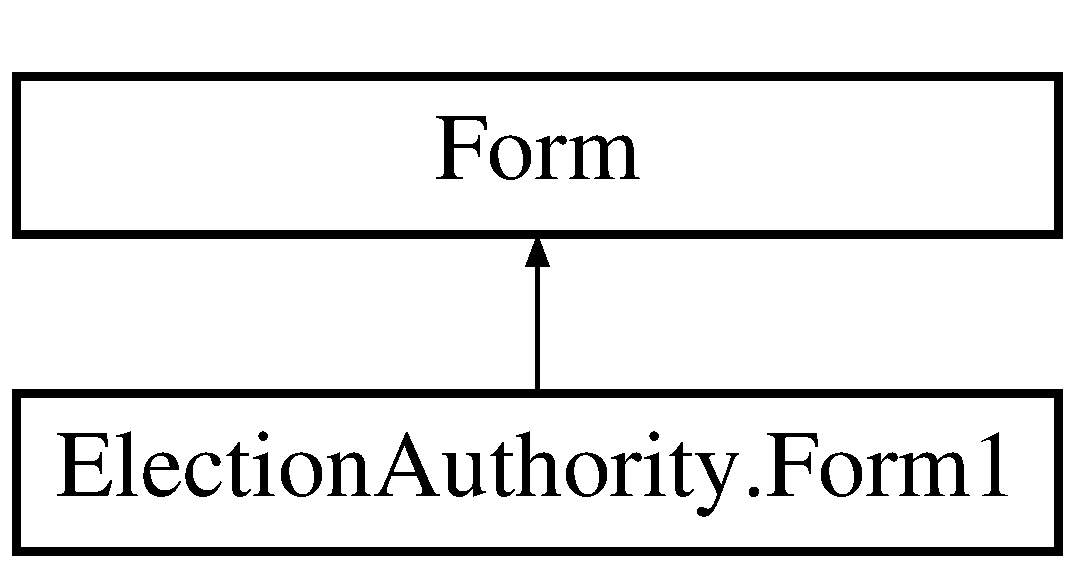
\includegraphics[height=2.000000cm]{class_election_authority_1_1_form1}
\end{center}
\end{figure}
\subsection*{Public Member Functions}
\begin{DoxyCompactItemize}
\item 
\hyperlink{class_election_authority_1_1_form1_a412d29d9ec02280ec1e7754ea34ab247}{Form1} ()
\begin{DoxyCompactList}\small\item\em constructor which creates Graphical User interface \end{DoxyCompactList}\item 
void \hyperlink{class_election_authority_1_1_form1_a82f9df8410a98e09ead89954fad7ebf1}{disable\+Send\+S\+L\+Tokens\+And\+Tokens\+Button} ()
\begin{DoxyCompactList}\small\item\em disable send\+S\+L\+And\+Tokens\+Button and enable finish\+Voting button \end{DoxyCompactList}\end{DoxyCompactItemize}
\subsection*{Protected Member Functions}
\begin{DoxyCompactItemize}
\item 
override void \hyperlink{class_election_authority_1_1_form1_a07a43432d6f1f2fab732f8f8db1aa3d3}{Dispose} (bool disposing)
\begin{DoxyCompactList}\small\item\em Clean up any resources being used. \end{DoxyCompactList}\end{DoxyCompactItemize}


\subsection{Detailed Description}
Class which shows a G\+U\+I 



\subsection{Constructor \& Destructor Documentation}
\hypertarget{class_election_authority_1_1_form1_a412d29d9ec02280ec1e7754ea34ab247}{}\index{Election\+Authority\+::\+Form1@{Election\+Authority\+::\+Form1}!Form1@{Form1}}
\index{Form1@{Form1}!Election\+Authority\+::\+Form1@{Election\+Authority\+::\+Form1}}
\subsubsection[{Form1}]{\setlength{\rightskip}{0pt plus 5cm}Election\+Authority.\+Form1.\+Form1 (
\begin{DoxyParamCaption}
{}
\end{DoxyParamCaption}
)\hspace{0.3cm}{\ttfamily [inline]}}\label{class_election_authority_1_1_form1_a412d29d9ec02280ec1e7754ea34ab247}


constructor which creates Graphical User interface 



\subsection{Member Function Documentation}
\hypertarget{class_election_authority_1_1_form1_a82f9df8410a98e09ead89954fad7ebf1}{}\index{Election\+Authority\+::\+Form1@{Election\+Authority\+::\+Form1}!disable\+Send\+S\+L\+Tokens\+And\+Tokens\+Button@{disable\+Send\+S\+L\+Tokens\+And\+Tokens\+Button}}
\index{disable\+Send\+S\+L\+Tokens\+And\+Tokens\+Button@{disable\+Send\+S\+L\+Tokens\+And\+Tokens\+Button}!Election\+Authority\+::\+Form1@{Election\+Authority\+::\+Form1}}
\subsubsection[{disable\+Send\+S\+L\+Tokens\+And\+Tokens\+Button}]{\setlength{\rightskip}{0pt plus 5cm}void Election\+Authority.\+Form1.\+disable\+Send\+S\+L\+Tokens\+And\+Tokens\+Button (
\begin{DoxyParamCaption}
{}
\end{DoxyParamCaption}
)\hspace{0.3cm}{\ttfamily [inline]}}\label{class_election_authority_1_1_form1_a82f9df8410a98e09ead89954fad7ebf1}


disable send\+S\+L\+And\+Tokens\+Button and enable finish\+Voting button 

\hypertarget{class_election_authority_1_1_form1_a07a43432d6f1f2fab732f8f8db1aa3d3}{}\index{Election\+Authority\+::\+Form1@{Election\+Authority\+::\+Form1}!Dispose@{Dispose}}
\index{Dispose@{Dispose}!Election\+Authority\+::\+Form1@{Election\+Authority\+::\+Form1}}
\subsubsection[{Dispose}]{\setlength{\rightskip}{0pt plus 5cm}override void Election\+Authority.\+Form1.\+Dispose (
\begin{DoxyParamCaption}
\item[{bool}]{disposing}
\end{DoxyParamCaption}
)\hspace{0.3cm}{\ttfamily [inline]}, {\ttfamily [protected]}}\label{class_election_authority_1_1_form1_a07a43432d6f1f2fab732f8f8db1aa3d3}


Clean up any resources being used. 


\begin{DoxyParams}{Parameters}
{\em disposing} & true if managed resources should be disposed; otherwise, false.\\
\hline
\end{DoxyParams}


The documentation for this class was generated from the following files\+:\begin{DoxyCompactItemize}
\item 
Election\+Authority/\+Election\+Authority/Form1.\+cs\item 
Election\+Authority/\+Election\+Authority/Form1.\+Designer.\+cs\end{DoxyCompactItemize}

\hypertarget{class_election_authority_1_1_logs}{}\section{Election\+Authority.\+Logs Class Reference}
\label{class_election_authority_1_1_logs}\index{Election\+Authority.\+Logs@{Election\+Authority.\+Logs}}


allows to collect and display logs  


\subsection*{Public Member Functions}
\begin{DoxyCompactItemize}
\item 
\hyperlink{class_election_authority_1_1_logs_a7a89ea08d448a21077c98adc82aa35ba}{Logs} (List\+View logs\+List\+View)
\begin{DoxyCompactList}\small\item\em \hyperlink{class_election_authority_1_1_logs}{Logs} instance\textquotesingle{}s constructor \end{DoxyCompactList}\item 
void \hyperlink{class_election_authority_1_1_logs_a8f630bd03f34e6c20a3fcc54535acfe2}{add\+Log} (string log, bool time, int flag, bool another\+Thread=false)
\begin{DoxyCompactList}\small\item\em adds log \end{DoxyCompactList}\end{DoxyCompactItemize}


\subsection{Detailed Description}
allows to collect and display logs 



\subsection{Constructor \& Destructor Documentation}
\hypertarget{class_election_authority_1_1_logs_a7a89ea08d448a21077c98adc82aa35ba}{}\index{Election\+Authority\+::\+Logs@{Election\+Authority\+::\+Logs}!Logs@{Logs}}
\index{Logs@{Logs}!Election\+Authority\+::\+Logs@{Election\+Authority\+::\+Logs}}
\subsubsection[{Logs}]{\setlength{\rightskip}{0pt plus 5cm}Election\+Authority.\+Logs.\+Logs (
\begin{DoxyParamCaption}
\item[{List\+View}]{logs\+List\+View}
\end{DoxyParamCaption}
)\hspace{0.3cm}{\ttfamily [inline]}}\label{class_election_authority_1_1_logs_a7a89ea08d448a21077c98adc82aa35ba}


\hyperlink{class_election_authority_1_1_logs}{Logs} instance\textquotesingle{}s constructor 


\begin{DoxyParams}{Parameters}
{\em logs\+List\+View} & logs list view\\
\hline
\end{DoxyParams}


\subsection{Member Function Documentation}
\hypertarget{class_election_authority_1_1_logs_a8f630bd03f34e6c20a3fcc54535acfe2}{}\index{Election\+Authority\+::\+Logs@{Election\+Authority\+::\+Logs}!add\+Log@{add\+Log}}
\index{add\+Log@{add\+Log}!Election\+Authority\+::\+Logs@{Election\+Authority\+::\+Logs}}
\subsubsection[{add\+Log}]{\setlength{\rightskip}{0pt plus 5cm}void Election\+Authority.\+Logs.\+add\+Log (
\begin{DoxyParamCaption}
\item[{string}]{log, }
\item[{bool}]{time, }
\item[{int}]{flag, }
\item[{bool}]{another\+Thread = {\ttfamily false}}
\end{DoxyParamCaption}
)\hspace{0.3cm}{\ttfamily [inline]}}\label{class_election_authority_1_1_logs_a8f630bd03f34e6c20a3fcc54535acfe2}


adds log 


\begin{DoxyParams}{Parameters}
{\em log} & log message\\
\hline
{\em time} & if print time\\
\hline
{\em flag} & type of message (error, info...)\\
\hline
{\em another\+Thread} & thread flag\\
\hline
\end{DoxyParams}


The documentation for this class was generated from the following file\+:\begin{DoxyCompactItemize}
\item 
Election\+Authority/\+Election\+Authority/Logs.\+cs\end{DoxyCompactItemize}

\hypertarget{class_election_authority_1_1_parser}{}\section{Election\+Authority.\+Parser Class Reference}
\label{class_election_authority_1_1_parser}\index{Election\+Authority.\+Parser@{Election\+Authority.\+Parser}}


parsing messages recived form clients  


\subsection*{Public Member Functions}
\begin{DoxyCompactItemize}
\item 
\hyperlink{class_election_authority_1_1_parser_a0bed6d110922dc3019536e8acf92caca}{Parser} (\hyperlink{class_election_authority_1_1_logs}{Logs} logs, \hyperlink{class_election_authority_1_1_election_authority}{Election\+Authority} election\+Authority)
\begin{DoxyCompactList}\small\item\em parser\textquotesingle{}s constructor \end{DoxyCompactList}\item 
bool \hyperlink{class_election_authority_1_1_parser_adb72772082dda3f1f124de0691670621}{parse\+Message} (string msg)
\begin{DoxyCompactList}\small\item\em parses message \end{DoxyCompactList}\end{DoxyCompactItemize}


\subsection{Detailed Description}
parsing messages recived form clients 



\subsection{Constructor \& Destructor Documentation}
\hypertarget{class_election_authority_1_1_parser_a0bed6d110922dc3019536e8acf92caca}{}\index{Election\+Authority\+::\+Parser@{Election\+Authority\+::\+Parser}!Parser@{Parser}}
\index{Parser@{Parser}!Election\+Authority\+::\+Parser@{Election\+Authority\+::\+Parser}}
\subsubsection[{Parser}]{\setlength{\rightskip}{0pt plus 5cm}Election\+Authority.\+Parser.\+Parser (
\begin{DoxyParamCaption}
\item[{{\bf Logs}}]{logs, }
\item[{{\bf Election\+Authority}}]{election\+Authority}
\end{DoxyParamCaption}
)\hspace{0.3cm}{\ttfamily [inline]}}\label{class_election_authority_1_1_parser_a0bed6d110922dc3019536e8acf92caca}


parser\textquotesingle{}s constructor 


\begin{DoxyParams}{Parameters}
{\em logs} & log instance\\
\hline
{\em election\+Authority} & election authority instance\\
\hline
\end{DoxyParams}


\subsection{Member Function Documentation}
\hypertarget{class_election_authority_1_1_parser_adb72772082dda3f1f124de0691670621}{}\index{Election\+Authority\+::\+Parser@{Election\+Authority\+::\+Parser}!parse\+Message@{parse\+Message}}
\index{parse\+Message@{parse\+Message}!Election\+Authority\+::\+Parser@{Election\+Authority\+::\+Parser}}
\subsubsection[{parse\+Message}]{\setlength{\rightskip}{0pt plus 5cm}bool Election\+Authority.\+Parser.\+parse\+Message (
\begin{DoxyParamCaption}
\item[{string}]{msg}
\end{DoxyParamCaption}
)\hspace{0.3cm}{\ttfamily [inline]}}\label{class_election_authority_1_1_parser_adb72772082dda3f1f124de0691670621}


parses message 


\begin{DoxyParams}{Parameters}
{\em msg} & recived message\\
\hline
\end{DoxyParams}
\begin{DoxyReturn}{Returns}
parsing result
\end{DoxyReturn}


The documentation for this class was generated from the following file\+:\begin{DoxyCompactItemize}
\item 
Election\+Authority/\+Election\+Authority/Parser.\+cs\end{DoxyCompactItemize}

\hypertarget{class_election_authority_1_1_permutation}{}\section{Election\+Authority.\+Permutation Class Reference}
\label{class_election_authority_1_1_permutation}\index{Election\+Authority.\+Permutation@{Election\+Authority.\+Permutation}}


represents all permutation\textquotesingle{}s method  


\subsection*{Public Member Functions}
\begin{DoxyCompactItemize}
\item 
\hyperlink{class_election_authority_1_1_permutation_a1bc4b8fbf2f81b64d4df43d842887f20}{Permutation} (\hyperlink{class_election_authority_1_1_logs}{Logs} logs)
\begin{DoxyCompactList}\small\item\em constructor \end{DoxyCompactList}\item 
List$<$ Big\+Integer $>$ \hyperlink{class_election_authority_1_1_permutation_aca696062c7feeb6e369163d85788f041}{generate\+Permutation} (int candidate\+Quantity)
\begin{DoxyCompactList}\small\item\em generate O\+N\+E permutation \end{DoxyCompactList}\item 
List$<$ Big\+Integer $>$ \hyperlink{class_election_authority_1_1_permutation_a986143acc7665192f2d5a577de873867}{get\+Inverse\+Permutation} (List$<$ Big\+Integer $>$ permutation)
\begin{DoxyCompactList}\small\item\em Find inverse permuatation using a table method \end{DoxyCompactList}\end{DoxyCompactItemize}


\subsection{Detailed Description}
represents all permutation\textquotesingle{}s method 



\subsection{Constructor \& Destructor Documentation}
\hypertarget{class_election_authority_1_1_permutation_a1bc4b8fbf2f81b64d4df43d842887f20}{}\index{Election\+Authority\+::\+Permutation@{Election\+Authority\+::\+Permutation}!Permutation@{Permutation}}
\index{Permutation@{Permutation}!Election\+Authority\+::\+Permutation@{Election\+Authority\+::\+Permutation}}
\subsubsection[{Permutation}]{\setlength{\rightskip}{0pt plus 5cm}Election\+Authority.\+Permutation.\+Permutation (
\begin{DoxyParamCaption}
\item[{{\bf Logs}}]{logs}
\end{DoxyParamCaption}
)\hspace{0.3cm}{\ttfamily [inline]}}\label{class_election_authority_1_1_permutation_a1bc4b8fbf2f81b64d4df43d842887f20}


constructor 


\begin{DoxyParams}{Parameters}
{\em logs} & logs instance\\
\hline
\end{DoxyParams}


\subsection{Member Function Documentation}
\hypertarget{class_election_authority_1_1_permutation_aca696062c7feeb6e369163d85788f041}{}\index{Election\+Authority\+::\+Permutation@{Election\+Authority\+::\+Permutation}!generate\+Permutation@{generate\+Permutation}}
\index{generate\+Permutation@{generate\+Permutation}!Election\+Authority\+::\+Permutation@{Election\+Authority\+::\+Permutation}}
\subsubsection[{generate\+Permutation}]{\setlength{\rightskip}{0pt plus 5cm}List$<$Big\+Integer$>$ Election\+Authority.\+Permutation.\+generate\+Permutation (
\begin{DoxyParamCaption}
\item[{int}]{candidate\+Quantity}
\end{DoxyParamCaption}
)\hspace{0.3cm}{\ttfamily [inline]}}\label{class_election_authority_1_1_permutation_aca696062c7feeb6e369163d85788f041}


generate O\+N\+E permutation 


\begin{DoxyParams}{Parameters}
{\em candidate\+Quantity} & quantity of candidates\\
\hline
\end{DoxyParams}
\begin{DoxyReturn}{Returns}

\end{DoxyReturn}
\hypertarget{class_election_authority_1_1_permutation_a986143acc7665192f2d5a577de873867}{}\index{Election\+Authority\+::\+Permutation@{Election\+Authority\+::\+Permutation}!get\+Inverse\+Permutation@{get\+Inverse\+Permutation}}
\index{get\+Inverse\+Permutation@{get\+Inverse\+Permutation}!Election\+Authority\+::\+Permutation@{Election\+Authority\+::\+Permutation}}
\subsubsection[{get\+Inverse\+Permutation}]{\setlength{\rightskip}{0pt plus 5cm}List$<$Big\+Integer$>$ Election\+Authority.\+Permutation.\+get\+Inverse\+Permutation (
\begin{DoxyParamCaption}
\item[{List$<$ Big\+Integer $>$}]{permutation}
\end{DoxyParamCaption}
)\hspace{0.3cm}{\ttfamily [inline]}}\label{class_election_authority_1_1_permutation_a986143acc7665192f2d5a577de873867}


Find inverse permuatation using a table method 


\begin{DoxyParams}{Parameters}
{\em permutation} & permutation to inverse\\
\hline
\end{DoxyParams}
\begin{DoxyReturn}{Returns}
inverse permutation
\end{DoxyReturn}


The documentation for this class was generated from the following file\+:\begin{DoxyCompactItemize}
\item 
Election\+Authority/\+Election\+Authority/Permutation.\+cs\end{DoxyCompactItemize}

\hypertarget{class_election_authority_1_1_serial_number_generator}{}\section{Election\+Authority.\+Serial\+Number\+Generator Class Reference}
\label{class_election_authority_1_1_serial_number_generator}\index{Election\+Authority.\+Serial\+Number\+Generator@{Election\+Authority.\+Serial\+Number\+Generator}}


Generates serial numbers used in E\+A  


\subsection*{Static Public Member Functions}
\begin{DoxyCompactItemize}
\item 
static List$<$ Big\+Integer $>$ \hyperlink{class_election_authority_1_1_serial_number_generator_ad035efa786ea1bce9edd67fe6b1ea7e8}{generate\+List\+Of\+Serial\+Number} (int number\+Of\+Serials, int number\+Of\+Bits)
\begin{DoxyCompactList}\small\item\em generate S\+L for election \end{DoxyCompactList}\item 
static List$<$ Asymmetric\+Cipher\+Key\+Pair $>$ \hyperlink{class_election_authority_1_1_serial_number_generator_acd0e3dda33ff955776c88c44c9e84976}{generate\+Pre\+Tokens} (int number\+Of\+Serials, int number\+Of\+Bits)
\begin{DoxyCompactList}\small\item\em generate pre tokens (key pair) for election \end{DoxyCompactList}\end{DoxyCompactItemize}


\subsection{Detailed Description}
Generates serial numbers used in E\+A 



\subsection{Member Function Documentation}
\hypertarget{class_election_authority_1_1_serial_number_generator_ad035efa786ea1bce9edd67fe6b1ea7e8}{}\index{Election\+Authority\+::\+Serial\+Number\+Generator@{Election\+Authority\+::\+Serial\+Number\+Generator}!generate\+List\+Of\+Serial\+Number@{generate\+List\+Of\+Serial\+Number}}
\index{generate\+List\+Of\+Serial\+Number@{generate\+List\+Of\+Serial\+Number}!Election\+Authority\+::\+Serial\+Number\+Generator@{Election\+Authority\+::\+Serial\+Number\+Generator}}
\subsubsection[{generate\+List\+Of\+Serial\+Number}]{\setlength{\rightskip}{0pt plus 5cm}static List$<$Big\+Integer$>$ Election\+Authority.\+Serial\+Number\+Generator.\+generate\+List\+Of\+Serial\+Number (
\begin{DoxyParamCaption}
\item[{int}]{number\+Of\+Serials, }
\item[{int}]{number\+Of\+Bits}
\end{DoxyParamCaption}
)\hspace{0.3cm}{\ttfamily [inline]}, {\ttfamily [static]}}\label{class_election_authority_1_1_serial_number_generator_ad035efa786ea1bce9edd67fe6b1ea7e8}


generate S\+L for election 


\begin{DoxyParams}{Parameters}
{\em number\+Of\+Serials} & number of serials to generate\\
\hline
{\em number\+Of\+Bits} & bit size of serial\\
\hline
\end{DoxyParams}
\begin{DoxyReturn}{Returns}
list of serial numbers
\end{DoxyReturn}
\hypertarget{class_election_authority_1_1_serial_number_generator_acd0e3dda33ff955776c88c44c9e84976}{}\index{Election\+Authority\+::\+Serial\+Number\+Generator@{Election\+Authority\+::\+Serial\+Number\+Generator}!generate\+Pre\+Tokens@{generate\+Pre\+Tokens}}
\index{generate\+Pre\+Tokens@{generate\+Pre\+Tokens}!Election\+Authority\+::\+Serial\+Number\+Generator@{Election\+Authority\+::\+Serial\+Number\+Generator}}
\subsubsection[{generate\+Pre\+Tokens}]{\setlength{\rightskip}{0pt plus 5cm}static List$<$Asymmetric\+Cipher\+Key\+Pair$>$ Election\+Authority.\+Serial\+Number\+Generator.\+generate\+Pre\+Tokens (
\begin{DoxyParamCaption}
\item[{int}]{number\+Of\+Serials, }
\item[{int}]{number\+Of\+Bits}
\end{DoxyParamCaption}
)\hspace{0.3cm}{\ttfamily [inline]}, {\ttfamily [static]}}\label{class_election_authority_1_1_serial_number_generator_acd0e3dda33ff955776c88c44c9e84976}


generate pre tokens (key pair) for election 


\begin{DoxyParams}{Parameters}
{\em number\+Of\+Serials} & number of serials to generate\\
\hline
{\em number\+Of\+Bits} & bit size of serial\\
\hline
\end{DoxyParams}
\begin{DoxyReturn}{Returns}
list of pre tokens
\end{DoxyReturn}


The documentation for this class was generated from the following file\+:\begin{DoxyCompactItemize}
\item 
Election\+Authority/\+Election\+Authority/Serial\+Number\+Generator.\+cs\end{DoxyCompactItemize}

\hypertarget{class_election_authority_1_1_server}{}\section{Election\+Authority.\+Server Class Reference}
\label{class_election_authority_1_1_server}\index{Election\+Authority.\+Server@{Election\+Authority.\+Server}}
\subsection*{Public Member Functions}
\begin{DoxyCompactItemize}
\item 
\hyperlink{class_election_authority_1_1_server_a60c4762524e5a2beb79b1305eb750ec6}{Server} (\hyperlink{class_election_authority_1_1_logs}{Logs} logs, \hyperlink{class_election_authority_1_1_election_authority}{Election\+Authority} election\+Authority)
\begin{DoxyCompactList}\small\item\em server which allows to communicate with other processes \end{DoxyCompactList}\item 
bool \hyperlink{class_election_authority_1_1_server_a24b27b5540dafbfc8e47d28e797daabe}{start\+Server} (string port)
\begin{DoxyCompactList}\small\item\em allow to start server \end{DoxyCompactList}\item 
void \hyperlink{class_election_authority_1_1_server_a4e68a6b5d8a483fe1f3064981558c2c5}{stop\+Server} ()
\begin{DoxyCompactList}\small\item\em stops server \end{DoxyCompactList}\item 
void \hyperlink{class_election_authority_1_1_server_ae7470865c5780cb90bf0ca53d6098f32}{send\+Message} (string name, string msg)
\begin{DoxyCompactList}\small\item\em sends message to client \end{DoxyCompactList}\end{DoxyCompactItemize}


\subsection{Constructor \& Destructor Documentation}
\hypertarget{class_election_authority_1_1_server_a60c4762524e5a2beb79b1305eb750ec6}{}\index{Election\+Authority\+::\+Server@{Election\+Authority\+::\+Server}!Server@{Server}}
\index{Server@{Server}!Election\+Authority\+::\+Server@{Election\+Authority\+::\+Server}}
\subsubsection[{Server}]{\setlength{\rightskip}{0pt plus 5cm}Election\+Authority.\+Server.\+Server (
\begin{DoxyParamCaption}
\item[{{\bf Logs}}]{logs, }
\item[{{\bf Election\+Authority}}]{election\+Authority}
\end{DoxyParamCaption}
)\hspace{0.3cm}{\ttfamily [inline]}}\label{class_election_authority_1_1_server_a60c4762524e5a2beb79b1305eb750ec6}


server which allows to communicate with other processes 


\begin{DoxyParams}{Parameters}
{\em logs} & allows to collect and display logs -\/ information in console\\
\hline
{\em election\+Authority} & represents class where is main logic of application\\
\hline
\end{DoxyParams}


\subsection{Member Function Documentation}
\hypertarget{class_election_authority_1_1_server_ae7470865c5780cb90bf0ca53d6098f32}{}\index{Election\+Authority\+::\+Server@{Election\+Authority\+::\+Server}!send\+Message@{send\+Message}}
\index{send\+Message@{send\+Message}!Election\+Authority\+::\+Server@{Election\+Authority\+::\+Server}}
\subsubsection[{send\+Message}]{\setlength{\rightskip}{0pt plus 5cm}void Election\+Authority.\+Server.\+send\+Message (
\begin{DoxyParamCaption}
\item[{string}]{name, }
\item[{string}]{msg}
\end{DoxyParamCaption}
)\hspace{0.3cm}{\ttfamily [inline]}}\label{class_election_authority_1_1_server_ae7470865c5780cb90bf0ca53d6098f32}


sends message to client 


\begin{DoxyParams}{Parameters}
{\em name} & name of client which we want to send a message\\
\hline
{\em msg} & message which we want to send\\
\hline
\end{DoxyParams}
\hypertarget{class_election_authority_1_1_server_a24b27b5540dafbfc8e47d28e797daabe}{}\index{Election\+Authority\+::\+Server@{Election\+Authority\+::\+Server}!start\+Server@{start\+Server}}
\index{start\+Server@{start\+Server}!Election\+Authority\+::\+Server@{Election\+Authority\+::\+Server}}
\subsubsection[{start\+Server}]{\setlength{\rightskip}{0pt plus 5cm}bool Election\+Authority.\+Server.\+start\+Server (
\begin{DoxyParamCaption}
\item[{string}]{port}
\end{DoxyParamCaption}
)\hspace{0.3cm}{\ttfamily [inline]}}\label{class_election_authority_1_1_server_a24b27b5540dafbfc8e47d28e797daabe}


allow to start server 


\begin{DoxyParams}{Parameters}
{\em port} & number of port on which server is running, this information comes from configuration xml file\\
\hline
\end{DoxyParams}
\begin{DoxyReturn}{Returns}
returns true when server started successfully
\end{DoxyReturn}
\hypertarget{class_election_authority_1_1_server_a4e68a6b5d8a483fe1f3064981558c2c5}{}\index{Election\+Authority\+::\+Server@{Election\+Authority\+::\+Server}!stop\+Server@{stop\+Server}}
\index{stop\+Server@{stop\+Server}!Election\+Authority\+::\+Server@{Election\+Authority\+::\+Server}}
\subsubsection[{stop\+Server}]{\setlength{\rightskip}{0pt plus 5cm}void Election\+Authority.\+Server.\+stop\+Server (
\begin{DoxyParamCaption}
{}
\end{DoxyParamCaption}
)\hspace{0.3cm}{\ttfamily [inline]}}\label{class_election_authority_1_1_server_a4e68a6b5d8a483fe1f3064981558c2c5}


stops server 



The documentation for this class was generated from the following file\+:\begin{DoxyCompactItemize}
\item 
Election\+Authority/\+Election\+Authority/Server.\+cs\end{DoxyCompactItemize}

%--- End generated contents ---

% Index
\backmatter
\newpage
\phantomsection
\clearemptydoublepage
\addcontentsline{toc}{chapter}{Index}
\printindex

\end{document}
